% !TEX root = ./main.tex
In figure \ref{fig:error}, we plot the mean error and standard deviation over 100 trajectories for a (scaled) Kalman gain. 
The $x$-axis denotes the scalar factor that the Kalman gain was multiplied by before computing the updated (a posteriori) state and covariance estimate. 

We can see in the table below that the results are relatively noisy, possibly attibuted to the large variance in state and measurement noise. 
However, the mean error is lowest for the Kalman filter, indicating that it is indeed optimal.

\begin{center}
    \begin{tabular}{ |p{2cm}||p{2cm}|p{4cm}|p{4cm}| }
    \hline
    \multicolumn{4}{|c|}{Mean error and standard deviation} \\
    \multicolumn{4}{|c|}{for scaled Kalman gain $a\cdot K$}\\
    \hline
    No.& $a$ & Mean Error & Standard Deviation \\
    \hline
    1 & 0.80 & 0.15626832 &          0.0834248\\
    2 & 0.84 & 0.15434268 &          0.0813475 \\
    3 & 0.88 & 0.153419 &            0.0824559   \\
    4 & 0.92 & 0.1520322 &           0.0827037 \\
    5 & 0.96 & 0.15366641 &          0.0838657 \\
    6 & 1.00 & \textbf{0.15154664} & 0.0802521 \\
    7 & 1.04 & 0.15273871 &          0.0852308 \\
    8 & 1.08 & 0.15204482 &          0.0835434 \\
    9 & 1.12 & 0.15206308 &          0.0814685 \\
    10 & 1.16 & 0.1536205 &          0.0826514 \\
    11 & 1.20 & 0.1588911 &          0.0836619 \\
    \hline
    \end{tabular}
    \end{center}

\begin{figure}[h]
    \centering
    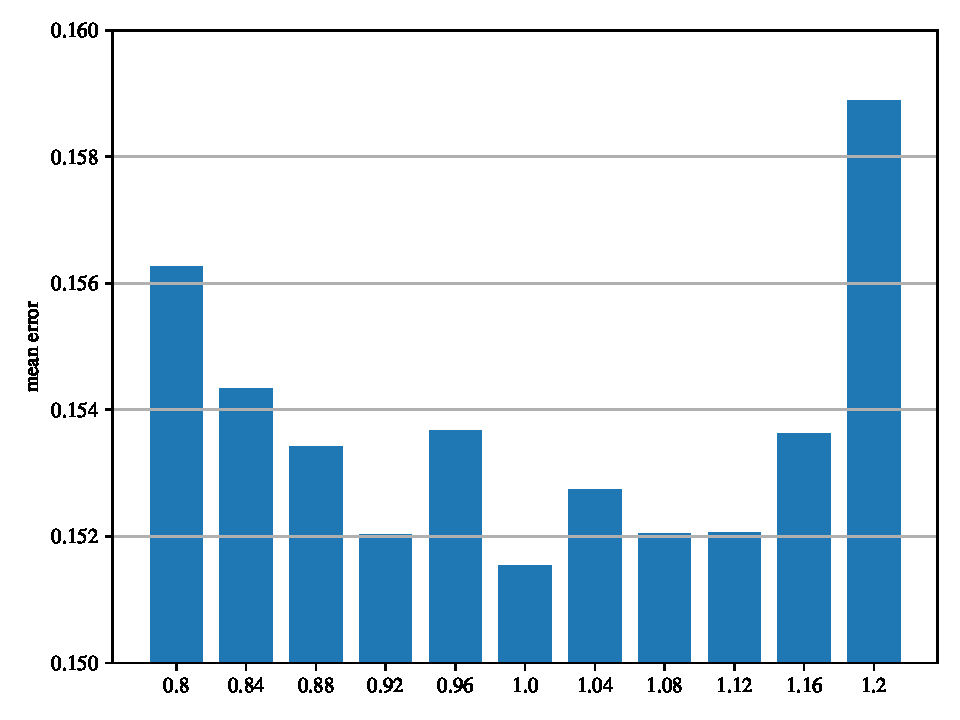
\includegraphics[width=\textwidth]{q3_2.pdf}
    \vspace{-5mm}
    \caption{Mean error and standard deviation over 100 trajectories for a (scaled) Kalman gain. The mean error is lowest for a scaling factor of 1 (i.e.~regular Kalman filter, indicating that it is indeed optimal).}
    \label{fig:error}
\end{figure}
\clearpage